\documentclass[aspectratio=169]{beamer}

% ---------- Packages ----------
\usepackage{amsmath, amsfonts, amssymb, bm}
\usepackage{booktabs}
\usepackage{tabularx}
\usepackage{tikz}
\usetikzlibrary{arrows.meta, positioning, shapes, calc}

% ---------- Theme ----------
\usetheme{Madrid}
\usecolortheme{default}

% ---------- Macros ----------
\newcommand{\norm}[1]{\left\lVert #1 \right\rVert}
\newcommand{\R}{\mathbb{R}}
\newcommand{\bbeta}{\bm{\beta}}

% ---------- Title info ----------
\title[L0 \& L1/2 Regularization]{L0 and L1/2 Regularization\\Sparsity Beyond L1}
\author{Team Name (A, B, C, D)}
\institute{Machine Learning}
\date{\today}

\begin{document}

% =========================================================
\begin{frame}
  \titlepage
\end{frame}

\begin{frame}{Outline}
  \tableofcontents
\end{frame}

% =========================================================
\section{Motivation: Why regularize?}

\begin{frame}{Why regularize? (Motivation)}
\begin{itemize}
  \item \textbf{Overfitting vs generalization:} training error decreases, test error may increase.
  \item \textbf{High-dimensional ML:} many features, noisy / correlated inputs.
  \item \textbf{Why we like sparsity:} interpretability, lower measurement cost, faster inference, robustness.
\end{itemize}
\vspace{0.5em}
\alert{Goal today:} encourage models with \textbf{few non-zero coefficients}.
\end{frame}

\begin{frame}{Overfitting picture (intuition)}
\centering
\begin{tikzpicture}[x=1cm,y=1cm]
  % Axes
  \draw[->] (0,0) -- (10,0) node[below right] {Model complexity};
  \draw[->] (0,0) -- (0,5) node[left] {Error};

  % Train curve (decreasing)
  \draw[thick] plot[smooth] coordinates {(0.8,4.2) (2,3.2) (4,2.2) (6,1.6) (8,1.2) (9.5,1.05)};
  \node[above] at (8.7,1.2) {Train};

  % Test curve (U-shape)
  \draw[thick,dashed] plot[smooth] coordinates {(0.8,4.0) (2,2.7) (4,1.7) (6,2.0) (8,3.0) (9.5,4.0)};
  \node[above] at (9.0,4.0) {Test};

  % Best point
  \fill (4,1.7) circle (2pt);
  \draw[dotted] (4,0) -- (4,1.7);
  \node[below] at (4,0) {$\lambda^\star$ (good bias/variance)};
\end{tikzpicture}

\vspace{0.6em}
\small Regularization controls complexity $\Rightarrow$ better generalization.
\end{frame}

% =========================================================
\section{Sparsity as a target}

\begin{frame}{What is sparsity?}
\begin{itemize}
  \item A model is \textbf{sparse} if many parameters are \textbf{exactly zero}.
  \item In linear models: $y \approx X\bbeta$, sparsity means only a few features are used.
  \item Benefits:
  \begin{itemize}
    \item interpretability (feature selection),
    \item lower cost (measure fewer features),
    \item deployment (faster + simpler models).
  \end{itemize}
\end{itemize}
\end{frame}

\begin{frame}{Sparsity illustration}
\centering
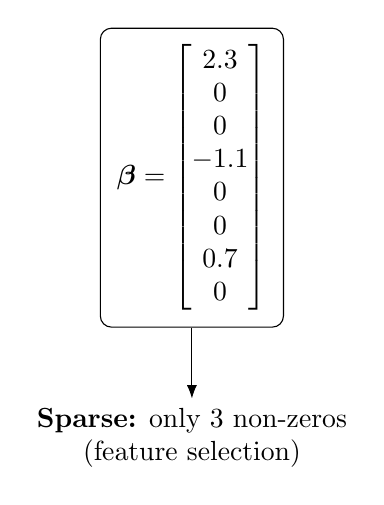
\begin{tikzpicture}[>=Latex]
  \node[draw, rounded corners, inner sep=6pt] (v) {$\bbeta = \begin{bmatrix}
  2.3\\ 0\\ 0\\ -1.1\\ 0\\ 0\\ 0.7\\ 0
  \end{bmatrix}$};

  \node[below=0.9cm of v, align=center] (t) {\textbf{Sparse:} only 3 non-zeros\\(feature selection)};
  \draw[->] (v) -- (t);
\end{tikzpicture}
\end{frame}

% =========================================================
\section{L0 regularization}

\begin{frame}{L0 regularization: definition}
\textbf{L0 “norm”} counts non-zero coefficients:
\[
\norm{\bbeta}_0 = \#\{j : \beta_j \neq 0\}.
\]

\textbf{Penalized objective:}
\[
\min_{\bbeta \in \R^p} \; \mathcal{L}(\bbeta) + \lambda \, \norm{\bbeta}_0
\]
where $\mathcal{L}(\bbeta)$ is the loss (e.g., MSE, logistic loss) and $\lambda>0$ controls sparsity.

\vspace{0.5em}
\alert{Interpretation:} “fit the data while using as few features as possible.”
\end{frame}

\begin{frame}{Intuition: best subset selection}
\begin{itemize}
  \item L0 regularization is closely related to \textbf{best subset selection}:
  \begin{itemize}
    \item choose a subset $S \subset \{1,\dots,p\}$,
    \item fit the model using only features in $S$,
    \item pick the best subset size (via $\lambda$ or $k$).
  \end{itemize}
  \item Often yields \textbf{very sparse} and \textbf{highly interpretable} models.
\end{itemize}
\end{frame}

\begin{frame}{Why L0 is hard}
\begin{itemize}
  \item The objective is \textbf{non-convex} and \textbf{discontinuous}.
  \item It implies a \textbf{combinatorial search} over feature subsets:
  \[
  \text{number of subsets} \approx 2^p.
  \]
  \item Practical consequence: exact optimization becomes infeasible when $p$ is large.
\end{itemize}
\end{frame}

\begin{frame}{How people handle L0 in practice}
Common strategies (choose depending on $p$ and compute budget):
\begin{itemize}
  \item \textbf{Greedy methods:} forward selection, Orthogonal Matching Pursuit (OMP).
  \item \textbf{Relaxations:} replace L0 by L1 (convex surrogate).
  \item \textbf{Mixed-Integer Optimization:} can solve exact/near-exact for smaller $p$.
  \item \textbf{Smooth surrogates:} continuous approximations to the counting function.
\end{itemize}
\end{frame}

% =========================================================
\section{L1/2 regularization}

\begin{frame}{L1/2 regularization: definition}
L1/2 is an $L_p$ penalty with $p=\tfrac{1}{2}$ (non-convex):
\[
\sum_{j=1}^p |\beta_j|^{1/2}.
\]

\textbf{Penalized objective:}
\[
\min_{\bbeta \in \R^p} \; \mathcal{L}(\bbeta) + \lambda \sum_{j=1}^p |\beta_j|^{1/2}.
\]

\vspace{0.4em}
\small Note: this is \textbf{not} Elastic Net (which is a mix of L1 and L2).
\end{frame}

\begin{frame}{Why L1/2 can be more sparse than L1}
\begin{itemize}
  \item For $p<1$, the penalty is \textbf{more aggressive near zero} than L1:
  \begin{itemize}
    \item small coefficients are pushed to exactly 0 more strongly,
    \item often yields \textbf{stronger sparsity} than L1.
  \end{itemize}
  \item Intuition often cited: \textbf{less shrinkage bias} on large coefficients than L1 (depends on solver/settings).
  \item Trade-off: \textbf{non-convex} objective $\Rightarrow$ optimization is harder.
\end{itemize}
\end{frame}

\begin{frame}{Optimization intuition (high-level)}
Typical solver families (no heavy math needed):
\begin{itemize}
  \item \textbf{Iterative reweighting:} solve a sequence of easier weighted problems that approximate L1/2.
  \item \textbf{Thresholding / proximal-style updates:} non-linear shrinkage rules.
\end{itemize}

Practical notes:
\begin{itemize}
  \item initialization matters,
  \item possible local minima (non-convex).
\end{itemize}
\end{frame}

% =========================================================
\section{Comparison and takeaways}

\begin{frame}{Comparison: L0 vs L1/2 vs L1}
\small
\begin{tabularx}{\textwidth}{lXXX}
\toprule
 & \textbf{L0} & \textbf{L1/2} & \textbf{L1} \\
\midrule
Sparsity strength & Very high (ideal) & High & Medium/High \\
Convex? & No (discrete) & No ($p<1$) & Yes \\
Optimization & Hard (combinatorial) & Hard/medium (non-convex) & Easier (convex) \\
Stability & Can be unstable & Depends on solver/init & Usually stable \\
Typical use-cases & Strict subset selection & Need more sparsity than L1 & Strong baseline, interpretable \\
\bottomrule
\end{tabularx}
\end{frame}

\begin{frame}{When to use what?}
\begin{columns}[T,onlytextwidth]
  \begin{column}{0.33\textwidth}
    \begin{block}{Use L1}
      \begin{itemize}
        \item Convex + reliable
        \item Good baseline
        \item Fast training
      \end{itemize}
    \end{block}
  \end{column}
  \begin{column}{0.34\textwidth}
    \begin{block}{Use L1/2}
      \begin{itemize}
        \item Need stronger sparsity
        \item Accept non-convexity
        \item Careful optimization
      \end{itemize}
    \end{block}
  \end{column}
  \begin{column}{0.33\textwidth}
    \begin{block}{Use L0}
      \begin{itemize}
        \item Strict feature subset
        \item Manageable $p$
        \item Specialized solvers
      \end{itemize}
    \end{block}
  \end{column}
\end{columns}
\end{frame}

\begin{frame}{Conclusion}
\begin{itemize}
  \item \textbf{L0:} direct sparsity objective, very interpretable, but computationally hard.
  \item \textbf{L1/2:} a bridge between L0 and L1; often yields stronger sparsity than L1, but non-convex.
  \item Always balance: \textbf{accuracy} vs \textbf{sparsity} vs \textbf{compute}.
\end{itemize}

\vspace{0.8em}
\centering
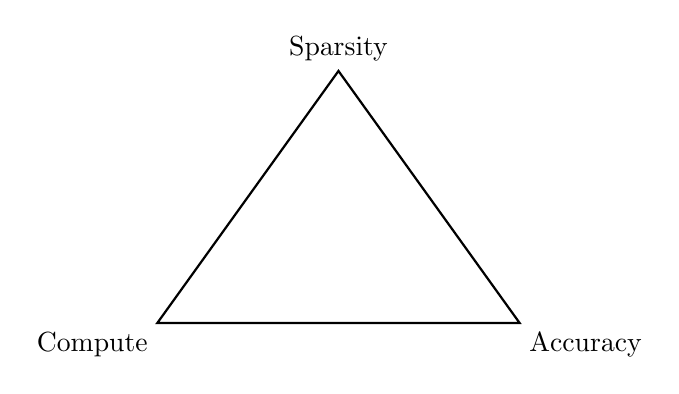
\begin{tikzpicture}[scale=1.0]
  \coordinate (A) at (0,0);
  \coordinate (B) at (4.6,0);
  \coordinate (C) at (2.3,3.2);
  \draw[thick] (A) -- (B) -- (C) -- cycle;
  \node[below left] at (A) {Compute};
  \node[below right] at (B) {Accuracy};
  \node[above] at (C) {Sparsity};
\end{tikzpicture}
\end{frame}

\begin{frame}{References (minimal)}
\small
\begin{itemize}
  \item Course notes / lecture slides on regularization and sparse modeling.
  \item Best subset selection / L0 regularization: classic regression model selection literature.
  \item Non-convex sparse penalties ($L_p$ with $p<1$): overview papers on non-convex regularization (optional).
\end{itemize}
\end{frame}

\end{document}

